\documentclass[conference]{IEEEtran}

\usepackage{graphicx}
\usepackage{algorithmicx}
\usepackage{algorithm}
\usepackage{algpseudocode}
\bibliographystyle{IEEEtran}

\newcommand{\tss}{\textsuperscript}

\title{HAZID Information Based Operational Procedure Diagnosis Method}

\author{\IEEEauthorblockN{Attila T\'{o}th} \IEEEauthorblockA{Computer and Automation \\ Research Institute\\ Budapest, Hungary\\ Email: atezs82@gmail.com} \and \IEEEauthorblockN{Katalin Hangos} \IEEEauthorblockA{Computer and Automation \\ Research Institute\\ Budapest, Hungary\\ Email: hangos@daedalus.scl.sztaki.hu} \and \IEEEauthorblockN{\'{A}gnes Werner-Stark} \IEEEauthorblockA{University of Pannonia\\ Veszpr\'{e}m, Hungary \\ Email: werner@virt.uni-pannon.hu}}

\begin{document}
\maketitle

\begin{abstract}

A novel fault diagnostic algorithm is presented in this paper based on the diagnostic idea described in \cite{KES:-:2011} for fault detection during operational procedure execution in  process systems. The basis of the method is an extension of a traditional HAZID methodology with procedural deviation information. A case study for demonstrating the capabilities of the algorithm on a simple example process system model with multiple operational procedures and multiple component faults is also presented.
 
\end{abstract}

\section{Introduction}
Detecting and diagnosing faults in complex process systems is an important task in ensuring safe operation and preventing losses. Albeit there had been results (\cite{original}) for detection of faults in steady-state process systems using hazard identification (HAZID), HAZOP and FMEA analysis results, but the transient case - when the plant is controlled by an operational procedure - is not addressed in them. The diagnostic idea described in \cite{KES-2011} offers a solution for this case. By extending the traditional HAZOP analysis with procedural deviations and root causes a novel way for searching component faults can be constructed. Using an appropriate comparison between reference and possibly faulty input-output event sequences of operational procedures a component fault can be diagnosed from the extended HAZOP analysis result. The algorithm formulated from this diagnostic idea is described in this paper. 

In the first part the basic notions which are used to describe and compare operational procedure executions with each other are collected, and the structure of the extended procedure HAZOP (procedure HAZID) analysis is described. Later the algorithm is formally defined and its capabilities are demonstrated using a simple case study. 

\section{Basic notions}

\subsection{Qualitative range spaces}
\label{sec:qualrngspc}
Current values of continuous outputs in process systems can be described using a properly selected qualitative range space. For example, to describe a value of a level sensor in a tank, the following range space can be used:

$\{\mathbf{e-},0,L,N,\mathbf{e+}\}$

Here $0$ means an empty tank, $L$ and $N$ means low and normal fluid level respectively, while $\mathbf{e-}$ and $\mathbf{e+}$ refer to unmeasurably low and high fluid levels (this might mean a failure in the level sensor itself). This range space will be used to describe system outputs during operation.

\subsection{Input-output event sequences}
\label{sec:ioseq}

Operational procedures in process systems are detailed list of instructions for the plant operator personnel to perform certain operations on the plant. Procedures can be formally described using finite input-output event sequences where one single event describes a change in either the inputs or the outputs of the system at a specific time instant. Therefore the syntax of a single input-output event is the following:

$event_x=(time-instant;{set~of~input~states};{set~of~output~states})$

The inputs in an event always refers to a state of an actuator component in the process system (eg. in the case of a valve it can be opened(1) or closed(0)). On the other hand, the outputs in an event refer to a value of an output of the process system in qualitative range using the qualitative set defined in section \ref{sec:qualrngspc}. Input-output event sequences are referred as traces later in the paper. As an example, a simple operational procedure can be described by the following trace over the inputs and the outputs of the system:

$(1;1,0;0) (2;1,0;L) (3;1,0;N) (4;1,1;N)$

For every operational procedure there exists a trace which describe its behavior under fault-free conditions. The method compares this trace to other traces which may have been executed under faulty conditions (called characteristic traces), these differences (called deviations) are later used to find possible malfunctions of components in the system.

\subsection{Deviations}
\label{sec:deviations}
Nominal and characteristic traces can be compared by comparing their correspoinding event fragments. Deviations are formed from a deviation guideword and the nominal event from which the corresponding characteristic trace event is deviating from. Two main deviation types can be distinguished.

\begin{itemize}
\item Temporal deviations. The input-output combination of the event did not happen exactly at the time instant as in the nominal event. 
	\begin{itemize}
	  \item $\mathbf{earlier}$ The event happened earlier in the characteristic trace.
	  \item $\mathbf{later}$ The event happened later in the characteristic trace.
	  \item $\mathbf{never-happened}$ The event never happened at all in the characteristic trace.
	\end{itemize}
\item Qualitative value deviations. The output of the event is different from the nominal event. The relational operators described in \cite{QUALCAL} to compare different qualitative values.
	\begin{itemize}
	  \item $\mathbf{greater}$ The output is greater in the characteristic trace.
	  \item $\mathbf{smaller}$ The output is smaller in the characteristic trace.
	\end{itemize}
\end{itemize}

It is possible to have both temporal and qualitative value deviations for a single difference. For example comparing nominal event $(1;0,1;L)$ with characteristic trace event $(1;0,1;0)$ might obviously lead to a $smaller(1;0,1;L)$ qualitative deviation, and it may lead to a $never-happened(1;0,1;L)$ temporal deviation if the characteristic trace does not contain the event $(1;0,1;L)$ at all (this might be the case when the tank has a leak and therefore it cannot fill up).

\subsection{Procedure HAZID}
\label{sec:prochazid}

As one type of traditional type of HAZID (HAZard IDentification) analysis, the HAZOP (HAZard and OPerability) analysis is widely used in the field of process system engineering to ensure operational safety during function. This analysis connects possible deviations of the measureable variables in the system with their causes and consequences under steady-state plant conditions. The results of such analysis are grouped by the type of the deviation (called "guideword") and are stored in a spreadsheet form (see table \ref{tab:ehazop}). 

As an other widely used and classical type of HAZID analysis, the FMEA (Fault Mode and Effect Analysis) analysis is initiated from failures in system subcomponents (called root causes), exploring the local and system-wide effects of these malfunctions, under steady-state plant conditions. As in the case of HAZOP, the results are kept in a spreadsheet (see table \ref{tab:efmea}). The combination of these two diagnostic approaches is not new (a method to find FMEA root causes from HAZOP measurable variable deviations is described in \cite{HAZOP-FMEA-ARTICLE}) but it had not been extended to operational procedure diagnosis.

Combining these diagnostic ideas in the domain of operational procedures, it becomes possible to connect deviations (as in HAZOP) between separate traces and acquire feasible component failures called root causes (as in FMEA). In such an extended analysis (called as procedure HAZID or  $\mathbf{P-HAZID}$, see table \ref{tab:eprochazid}) a chain of deviations (see \ref{sec:deviations}) can be set up to by matching deviations of the "Cause" and "Deviation" column with their equal counterparts in the "Cause" and "Implication" column for a different row. If the analysis is consistent, then all of these deviation chains lead to a root cause which indicate specific component failures (eg. rupture of the tank) provided all deviations in the chain are present between an observed and a reference trace (described in section \ref{sec:deviations}). Following all possible deviation chains based on the collected deviations a set of possible component failures can be found given a properly defined $\mathbf{P-HAZID}$ table. 

It was assumed that component failures were static, and happened before the execution of the procedure has begun. Therefore, unlike in the case of deviations, time instants were not assigned to them. The component failures were not connected to any input or output values in any direct way, so these values had been also omitted from their definition. 

\begin{table}
\label{tab:ehazop}
\caption{A simple example of a HAZOP table}
\begin{tabular}{|l|l|l|l|}
\hline
Guideword & Deviation & Causes & Consequences \\
\hline
\hline
low & LEVEL low & LOW input & LOW output \\
& LEVEL low & TANK rupture & LOW output \\
\hline
high & LEVEL high & HIGH input & TANK rupture \\
\hline
\end{tabular}
\end{table}

\begin{table*}
\centering
\label{tab:efmea}
\caption{A simple example of an FMEA table}
\begin{tabular}{|l|l|l|l|l|}
\hline
Component & Failure mode & Failure mode causes & Local effects & System effects \\
\hline
\hline
TANK & leaking & rupture & LOW tank output & escaping fluid \\
\hline
OUTPUT VALVE & close failure & broken & LOW fluid level & output tank cannot be changed \\
\hline
\end{tabular}
\end{table*}

\begin{table*}
\centering
\label{tab:eprochazid}
\caption{A simple example of a P-HAZID table}
\begin{tabular}{|l|l|l|}
\hline
Cause & Deviation & Implication \\
\hline
\hline
TANK-LEAK & never-happened(2;1,0,L) & never-happened(3;1,0,N) \\
\hline
never-happened(2;1,0,L) & never-happened(3;1,0,N) & never-happened(4;1,1,N) \\
\hline
TANK-LEAK & smaller(2;1,0,L) & smaller(3;1,0,N) \\
\hline
smaller(2;1,0,L) & smaller(3;1,0,N) & smaller(4;1,1,N) \\
\hline
POS-BIAS & greater(1;1,0,0) & greater(2;1,0,L) \\
\hline
greater(1;1,0,0) & greater(2;1,0,L) & greater(3;1,0,N) \\
\hline
greater(2;1,0,L) & greater(3;1,0,N) & never-happened(4;1,1,N) \\
\hline
POS-BIAS& never-happened(1;1,0,0) & earlier(2;1,0,L) \\
\hline
never-happened(1;1,0,0) & earlier(2;1,0,L) & earlier(3;1,0,N) \\
\hline
\end{tabular}
\end{table*}

The algorithm uses this technique first to find possible  $\mathbf{P-HAZID}$ row(s) to start from (from the set of initial deviations), then following the deviation chains defined by these rows towards a possible root cause, traversing new rows based on the initial set of deviations. Using this procedure, it may end up at a root cause, or at a row with deviations from which it cannot proceed forward - because they are not contained in the initial set of deviations. 

If the $\mathbf{P-HAZID}$ table is inconsistent (not all deviation sequences lead to root causes) then it may end up at a row from where it cannot proceed forward, therefore the algorithm can be used for validation purposes, too. 

%
\section{Diagnosis Using Observed Event Sequences and Procedure HAZID}
\label{sec:reasoning}

As described in section \ref{sec:prochazid}, the diagnosis is based on the fact that a row in the $\mathbf{P-HAZID}$
table can be interpreted as one of the rules below:
\begin{small}
\begin{eqnarray*}
&& If~~\mathbf{(Cause,Deviation)}~~then~~\mathbf{Implication} \\
&& If~~\mathbf{(Cause)}~~then~~\mathbf{(Deviation,Implication})
\end{eqnarray*}
\end{small}
\noindent where all of the \textbf{Cause}, \textbf{Deviation} and \textbf{Implication}
 are predicates
 defined by the deviation of events or by the plant component failure modes
present in the corresponding columns of the table (see an example in table \ref{tab:eprochazid}).
Note that a pair of predicates is used for both the forward reasoning
 applying the first rule form, and to the backward one with the second rule form.

\floatname{algorithm}{Algorithm}
 
The algorithm attempts to find the root causes, if there are any, based on the following input:
\begin{itemize}
	\item $\mathbf{P-HAZID}$ table (as a spreadsheet) The table is assumed not to contain duplicate rows containing the same "cause", "deviation" and "implication" triplet.
	\item Nominal trace ($\mathbf{nominalTrace}$) as a timed event sequence as in section \ref{sec:ioseq}. It is assumed that the number of events in the nominal trace is not less than 2.
	\item Characteristic trace ($\mathbf{chrTrace}$) as a timed event sequence as in section \ref{sec:ioseq}.
\end{itemize}

The output is a set of identified root causes ($\mathbf{IRC}$) and identified non-root causes ($\mathbf{INC}$) for the analysis trace. The procedure attempts to identify the root causes using a search of Algorithm \ref{alg:main}. If such root causes are found, they are appended to the set of ($\mathbf{IRC}$). If the algorithm cannot perform the search onwards from a specific non-root cause, then this cause is added to the set of ($\mathbf{INC}$). This can happen either because of the $\mathbf{P-HAZID}$ table is incomplete or the cause to continue the search with is not present in the set of deviations. Both output sets might be empty, when there are no deviations (a nominal trace is provided as an input to the algorithm).

The notations which are used in the description of the algorithm are defined as follows:

\begin{itemize}
\item Precedence. Let the notation $(event_x) \prec (event_y)$ mean that $event_x$ precedes $event_y$ in a trace in time.
\item All root causes. Let the set $\mathbf{RC}$ contain all possible root causes for the provided $\mathbf{P-HAZID}$ table. The root causes can be acquired from the provided $\mathbf{P-HAZID}$ table by collecting all elements from the "Cause" column which are not deviatons.
\item Cell reference in the HAZID table. Let the value $cause(R)$, $dev(R)$ and $imp(R)$ refer to the ordering relations of the corresponding column
in the $\mathbf{P-HAZID}$ table at row number $R$.
\item Deviation containment. Let $\mathbf{DEV}$ be a set of $(time)\times(deviation)$. In this sense let the notation $cause(R) \in \mathbf{DEV}$ mean that $cause$ is an element of $\mathbf{DEV}$ for an arbitrary $time$.
\item Accessing events. Let $eventSequence(time)$ refer to the $event$ happened at time $time$ in $eventSequence$.
\item Sequence length. Let $length(eventSequence)$ refer to the number of events in the sequence.
\item Projection. If $pair = (p,q)$ is an ordered pair then let $proj_1(pair)=p$ and $proj_2(pair)=q$.
\item Set containment. If $\mathbf{a} \in \mathbf{SET}$ then the operation $\mathbf{SET} \leftarrow \mathbf{SET} \bigcup \mathbf{a}$ has no effect, every element may present only once in a set.
\end{itemize}

The algorithm is described in Algorithm \ref{alg:main} in detail. First all deviations along with their time instances are collected and stored in $\mathbf{DEV}$. Devations are formed when an event in the observed trace is deviating from its nominal correspondent, according to the ordering relations listed in section \ref{sec:deviations}. Sets $\mathbf{INC}$ and $\mathbf{IRC}$ are given empty initial values. The set of final deviation pairs ($\mathbf{FDP}$) is also calculated, this set contains all deviations of $\mathbf{chrTrace}$ from $\mathbf{nominalTrace}$ at the last and its preceding time instant where deviations are present as ordered pairs. The end of the characteristic trace is not neccessarily deviating from the nominal trace, therefore the deviation pair from which the reasoning can be initiated might not be situated the final and preceding time instant. After the initialization, a recursive reasoning procedure is initiated on the $\mathbf{P-HAZID}$ table using the $\mathbf{FDP}$ set as a starting point.

The core of the recursion checks the \textit{deviation} and \textit{implication} rows in the $\mathbf{P-HAZID}$ table and accoring to the corresponding \textit{cause} value it
\begin{enumerate}
\item either, if \textit{cause} is a root cause then adds it to the list of root causes $\mathbf{IRC}$ and returns
\item or, if \textit{cause} is a non-root cause but it cannot continue the search it adds \textit{cause} to the list of non-root causes $\mathbf{INC}$ and returns
\item or, if \textit{cause} is a non-root cause and it can continue the search then it moves to a correponding next row in the $\mathbf{P-HAZID}$ table by calling itself recursively.
\end{enumerate}

The algorithm stops with the reasoning because of either the corresponding cause (with which the search need to be continued):
\begin{enumerate}
\item does not present in the set of deviations prior to the actual deviation,
\item or, with its corresponding implication does not exist in the $\mathbf{P-HAZID}$ table for any row as implication and deviation. The $\mathbf{P-HAZID}$ table is not complete in this case.
\end{enumerate}

In either cases the algorithm adds the cause to the set of $\mathbf{INC}$ and moves on with the next possible final deviation pair, if available.

\begin{algorithm*}
\caption{Recursive reasoning procedure}
\label{alg:main}
\begin{algorithmic}[1]
\State $\mathbf{DEV} \leftarrow \{ \emptyset \}$
\State $\mathbf{t^*}=length(nominalTrace)$
\For{$T:=1$ to $length(\mathbf{t^*})$}
\ForAll{deviation $D$ of $chrTrace$ from $nominalTrace$ at time $T$}
\State $\mathbf{DEV} \leftarrow \mathbf{DEV} \bigcup (T,D)$
\EndFor
\EndFor
\State $\mathbf{INC} \leftarrow \{ \emptyset \}$
\State $\mathbf{IRC} \leftarrow \{ \emptyset \}$
\State $\mathbf{t_{FDP}}$=$\{ \exists \mathbf{t}, \exists d_1, \exists d_2, (\mathbf{t},d_1) \in \mathbf{DEV}, (\mathbf{t-1},d_2) \in \mathbf{DEV} \}$
\State $\mathbf{FDP} \leftarrow \{(\forall d_1,\forall d_2 (\mathbf{t_{FDP}-1},d1) \in \mathbf{DEV},(\mathbf{t_{FDP}},d2) \in \mathbf{DEV}, (\mathbf{t_{FDP}-1},d_1) \times (\mathbf{t_{FDP}},d_2) \}$ 
\ForAll{$pair \in \mathbf{FDP}$}
  \State $startDeviation \leftarrow proj_1(pair)$
  \State $startImplication \leftarrow proj_2(pair)$
  \State \Call {step}{startDeviation, startImplication}
\EndFor
\Procedure{step}{deviation,implication}
 \If{$\exists R,deviation=dev(R),implication=imp(R)$}
  \ForAll{$ \{ R,dev(R)=deviation~\mathbf{and}~imp(R)=implication \} $}
   \If{$cause(R) \in \mathbf{RC}$}
     \State $\mathbf{IRC} \leftarrow \mathbf{IRC} \bigcup cause(R)$
     \State \Return
   \Else
     \If{$cause(R) \in \mathbf{DEV}~\mathbf{and}~cause(R) \prec dev(R)~in~\mathbf{DEV}$}
          	\State \Call {step}{cause(R), dev(R)}
     \Else
      \State $\mathbf{INC} \leftarrow \mathbf{INC} \bigcup cause(R)$
      \State \Return
     \EndIf
   \EndIf
 \EndFor
\Else
\State $\mathbf{INC} \leftarrow \mathbf{INC} \bigcup cause(R)$
      \State \Return
\EndIf
\EndProcedure
\end{algorithmic}
\end{algorithm*}

After the recursion finished, set $\mathbf{IRC}$ contains the set of identified root causes, while the set
$\mathbf{INC}$ contain the set of deviations which might lead to a failure but either do not occur in the list
of deviations in advance of the actual deviation or the search could not find any row in the $\mathbf{P-HAZID}$ table with which it could move forward.

\subsection{Example sets}
\label{sec:exsets}

For example, for nominal trace 

$(1;1,0;0) (2;1,0;L) (3;1,0;N) (4;1,1;N)$

and characteristic trace 

$(1;1,0;0) (2;1,0;0) (3;1,0;0) (4;1,1;0)$

the working sets of the algorithm are calculated as it can be seen on table \ref{tbl:algVariables}.

\begin{table*}
\centering
\label{tbl:algVariables}
\begin{tabular}{p{12cm}}
\hline
   $\mathbf{DEV} \leftarrow \{ never-happened(2;0,1;L),never-happened(3;0,1;L),$ \\ 
   $never-happened(4;1,1;N),smaller(2;0,1;L),smaller(3;0,1;N),$
   $smaller(4;1,1;N) \}$ \\
   $\mathbf{FDP} \leftarrow \{ (smaller(3;0,1;N),never-happened(3;0,1;N),$\\
   $smaller(4;0,1;N),never-happened(4;0,1;N) $ \\   

   $\mathbf{IRC} \leftarrow \{ TANK-LEAK, VA1-CONGESTION \}$ \\
   $\mathbf{INC} \leftarrow \{ smaller(1;1,0;0),later(2;1,0;L)\}$ \\
\hline
\end{tabular}
\caption{Sets of the case study in section \ref{sec:exsets} }
\end{table*}

\section{Implementation}
The algorithm was implemented in Java and uses a simple XML format for parsing the nominal and the characteristic trace and the $\mathbf{P-HAZID}$ spreadsheet. During execution the following information is printed out to the console:

\begin{itemize}
\item The parsed nominal, characteristic trace and $\mathbf{P-HAZID}$ spreadsheet.
\item Set of deviations between the nominal and characteristic trace.
\item Set of deviation pairs used to start the reasoning procedure.
\item Set of paths which either lead to a root cause or a non-root cause.
\item Set of identified root and non-root causes.
\end{itemize}

\section{Case Study}

\subsection{Process system}
\label{sec:procsys}

In the case study the simple process system of figure \ref{fig:tank} was used to evaluate the algorithm. It consists of a fluid tank, an input (VA1) and an output (VA2) valve and a level sensor (LI), therefore it has two boolean inputs (the state of the valves, open or closed) and a single qualitative output, the value of the level sensor. For the sake of simplicty, boolean valve states and a reduced qualitative range (see section \ref{sec:qualrngspc}) was used, but it could have been possible to use more input states and a broader qualitative range (these issues will be addressed in \ref{sec:discussion}). 

\begin{figure}[h!]
 \begin{center}
  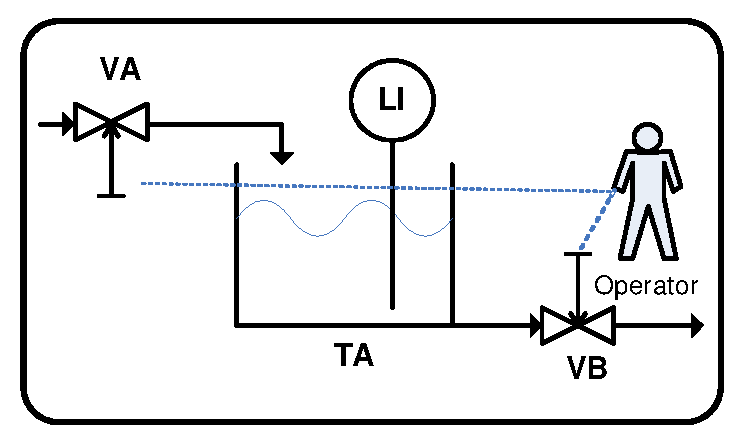
\includegraphics[width=6cm]{Stank.eps}
  \caption {Supply tank with inflow and outflow valve and level sensor}
  \label{fig:tank}
 \end{center}
\end{figure} 

The component faults were always single and static during the execution of the operational procedures. The following malfunctions were used:
\begin{enumerate}
\item The leak of the tank. On the leak the fluid loss over time was equal to what caused by the open output (VA2) valve.
\item Input (VA1) or output (VA2) valve close failure (valve cannot be closed).
\item Input (VA1) or output (VA2) valve congestion (no fluid could pass the valve).
\item Additive positive or negative bias of the tank level sensor LI. The sensor was measuring values in qualitative range $\{\mathbf{e-},0,L\}$ in the negative bias case and $\{L,N,\mathbf{e+}\}$ in the positive bias case (see section \ref{sec:qualrngspc} for the whole range).
\end{enumerate}

\subsection{Operational procedures}

These simple operational procedures were collected for the process system:
\begin{itemize}
\item Normal operation. Describes a normal operation of the system. The tank is filled using the input valve, then the output valve is opened. The corresponding nominal trace:
$(1;1,0;0) (2;1,0;L) (3;1,0,N) (4;1,1,N)$
\item Maintenance empty procedure. Describes a maintenance procedure when all fluid is removed from the system through the output valve. The corresponding nominal trace:
$(1;0,1;N) (2;0,1;L) (3;0,1;0) (4;0,0;0)$
\item Tank fill procedure. Describes a special procedure when the tank is filled with fluid and then the input valve is closed. The corresponding nominal trace:
$(1;1,0;0) (2;1,0;L) (3;1,0;N) (4;0,0;N)$
\end{itemize}

The $\mathbf{P-HAZID}$ table containing the fault root causes based on the faulty traces were created for each operational procedure. For the "Normal operational procedure" the table is presented in Table \ref{tab:normalophazid}.

\begin{table*}
\centering
\label{tab:normalophazid}
\begin{tabular}{|l|l|l|}
\hline
Cause & Deviation & Implication \\
\hline
TANK-LEAK & never-happened(2;1,0,L) & never-happened(3;1,0,N) \\
never-happened(2;1,0,L) & never-happened(3;1,0,N) & never-happened(4;1,1,N) \\
TANK-LEAK & smaller(2;1,0,L) & smaller(3;1,0,N) \\
smaller(2;1,0,L) & smaller(3;1,0,N) & smaller(4;1,1,N) \\
POS-BIAS & greater(1;1,0,0) & greater(2;1,0,L) \\
greater(1;1,0,0) & greater(2;1,0,L) & greater(3;1,0,N) \\
greater(2;1,0,L) & greater(3;1,0,N) & never-happened(4;1,1,N) \\
POS-BIAS & never-happened(1;1,0,0) & earlier(2;1,0,L) \\
never-happened(1;1,0,0) & earlier(2;1,0,L) & earlier(3;1,0,N) \\
earlier(2;1,0,L) & earlier(3;1,0,N) & never-happened(4;1,1,N) \\
NEG-BIAS & smaller(1;1,0,0) & smaller(2;1,0,L) \\
smaller(1;1,0,0) & smaller(2;1,0,L) & smaller(3;1,0,N) \\
smaller(2;1,0,L) & smaller(3;1,0,N) & smaller(4;1,1,N) \\
NEG-BIAS & later(1;1,0,0) & later(2;1,0,L) \\
later(1;1,0,0) & later(2;1,0,L) & never-happened(3;1,0,N) \\
later(2;1,0,L) & never-happened(3;1,0,N) & never-happened(4;1,1,N) \\
VA1-CONGESTION & smaller(2;1,0,L) & smaller(3;1,0,N) \\
smaller(2;1,0,L) & smaller(3;1,0,N) & smaller(4;1,1,N) \\
VA2-CONGESTION & never-happened(4;1,1,N) & not available \\
VA2-CONGESTION & greater(4;1,1,N) & not available \\
\hline
\end{tabular}
\caption{Normal operational procedure P-HAZID table}
\end{table*}

\subsection{Results}

After executing the algorithm on the nominal and faulty traces and the $\mathbf{P-HAZID}$ table, the following identified root causes ($\mathbf{IRC}$) and non-identified root causes ($\mathbf{INC}$) were obtained using the algorithm with the "Normal operational procedure" during the presence of the single failures (refer to subsection \ref{sec:procsys}).

\begin{itemize}

\item Fault TANK-LEAK: \\ $\mathbf{IRC} \leftarrow \{ TANK-LEAK,VA1-CONGESTION \} $\\ $\mathbf{INC} \leftarrow \{ smaller(1;1,0;0), later(2;1,0;L) \}$

\item Fault VA1-CONGESTION: \\ $\mathbf{IRC} \leftarrow \{ TANK-LEAK,VA1-CONGESTION \}$\\ $\mathbf{INC} \leftarrow \{ smaller(1;1,0;0), later(2;1,0;L) \}$

\item Fault VA2-CONGESTION: Too few deviations, fault could not be detected.

\item Fault VA1-CLOSE-FAILURE: Trace was identical, fault could not be detected.

\item Fault VA2-CLOSE-FAILURE: Trace was identical, fault could not be detected.

\item Fault POS-BIAS: \\ $\mathbf{IRC} \leftarrow \{ POS-BIAS \}$ \\ $\mathbf{INC} \leftarrow \{ \emptyset \} $

\item Fault NEG-BIAS: \\ $\mathbf{IRC} \leftarrow \{ TANK-LEAK, NEG-BIAS, VA1-CONGESTION \}$ \\ $\mathbf{INC} \leftarrow \{ never-happened(2;1,0;L) \}$

\end{itemize}

Similar results were obtained after executing the algorithm for the other operational procedures.

\subsection{Discussion}
\label{sec:discussion}

The case study proved that the diagnostic algorithm produced the expected results in the simple case of process system described in section \ref{sec:procsys}, and the following observations were made:

\begin{enumerate}
\item When the faulty trace generates very representative deviations then the algorithm is accurate, it gives the real root cause with no spurious or unresolved causes (in the case of POS-BIAS).
\item When the faulty trace is identical to the nominal or too few deviations can be found, then faults cannot be diagnosed (in the case of VA2-CONGESTION, VA1-CLOSE-FAILURE or VA2-CLOSE-FAILURE).
\item Obviously, when faults are present in component functionality which is not used (in the case of VA1-CLOSE-FAILURE or VA2-CLOSE-FAILURE) then these faults remain undetectable.
\item When faults have similar effects on the system (in the case of VA1-CONGESTION and TANK-LEAK), then faults are detectable, albeit they cannot be distinguished from each other and both of them are present in the result set.
\end{enumerate}

In order to increase the accurancy of the diagnostic algorithm, the following improvements could be made to the model of the process system:
\begin{enumerate}
\item Increase the size of the qualitative range (and trace length at the same time). This will result in a greater (more representative) set of deviations and the HAZID table will contain more accurate (more unique) paths to failures.
\item Increase the granularity of the qualitative comparison operators (SMALLER and GREATER type deviations). This will make differences in the qualitative deviations distinguishable.
\item Increase the number of analysed outputs in the system (for example measure an overflow sensor of the tank as well). Increased number of outputs in the HAZID table might yield to an increased accurancy in finding the root cause. In this case the algorithm need to be improved to handle this scenario.
\end{enumerate}

\section {Conclusion and Future work}
A novel diagnostic algorithm for diagnosing faults in process systems during operational procedure execution has been described in this paper. The algorithm is based on the fault diagnostic idea described in \cite{KES2011} extending the traditional HAZOP process system diagnostic methodology for operational procedures. It had been implemeneted in Java and uses a simple XML data format as input for the procedures and additional HAZID information. A case study in a simple test process system is presented with appropriate results, and ways for further improvement were collected in \ref{sec:discussion}.

It would be benefical to evaluate the method on a more complex process system with more outputs and increased qualitative range on them. An appropriate process system need to be selected, and simulations need to be executed to acquire traces under nominal and faulty conditions and create the $\mathbf{P-HAZID}$ table. The algorithm itself should be extended as well to handle multiple outputs.

The method could be extended to work on real-time trace deviation data instead of offline source, in this case significant modifications need to be implemented but the applicability of the algorithm would be greatly increased.

\section{Acknowledgements} 
We acknowledge the financial support of this work by the Hungarian State and the European Union under the TAMOP-????? project and by the Hungarian Scientific Research Fund through
grants K83440.

\end{document}